\documentclass[8pt]{beamer}

% Beamer style
%\usetheme[secheader]{Madrid}
% \usetheme{CambridgeUS}
\useoutertheme{infolines}
\usecolortheme[rgb={0.65,0.15,0.25}]{structure}
% \usefonttheme[onlymath]{serif}
\beamertemplatenavigationsymbolsempty
%\AtBeginSubsection

% Packages
%\usepackage[french]{babel}
\usepackage[latin1]{inputenc}
\usepackage{color}
\usepackage{xspace}
\usepackage{dsfont, stmaryrd}
\usepackage{amsmath, amsfonts, amssymb, stmaryrd}
\usepackage{epsfig}
\usepackage{tikz}
\usepackage{url}
% \usepackage{ulem}
\usepackage{/home/robin/LATEX/Biblio/astats}
%\usepackage[all]{xy}
\usepackage{graphicx}
\usepackage{xspace}

% Maths
% \newtheorem{theorem}{Theorem}
% \newtheorem{definition}{Definition}
\newtheorem{proposition}{Proposition}
% \newtheorem{assumption}{Assumption}
% \newtheorem{algorithm}{Algorithm}
% \newtheorem{lemma}{Lemma}
% \newtheorem{remark}{Remark}
% \newtheorem{exercise}{Exercise}
% \newcommand{\propname}{Prop.}
% \newcommand{\proof}{\noindent{\sl Proof:}\quad}
% \newcommand{\eproof}{$\blacksquare$}

% \setcounter{secnumdepth}{3}
% \setcounter{tocdepth}{3}
\newcommand{\pref}[1]{\ref{#1} p.\pageref{#1}}
\newcommand{\qref}[1]{\eqref{#1} p.\pageref{#1}}

% Colors : http://latexcolor.com/
\definecolor{darkred}{rgb}{0.65,0.15,0.25}
\definecolor{darkgreen}{rgb}{0,0.4,0}
\definecolor{darkred}{rgb}{0.65,0.15,0.25}
\definecolor{amethyst}{rgb}{0.6, 0.4, 0.8}
\definecolor{asparagus}{rgb}{0.53, 0.66, 0.42}
\definecolor{applegreen}{rgb}{0.55, 0.71, 0.0}
\definecolor{awesome}{rgb}{1.0, 0.13, 0.32}
\definecolor{blue-green}{rgb}{0.0, 0.87, 0.87}
\definecolor{red-ggplot}{rgb}{0.52, 0.25, 0.23}
\definecolor{green-ggplot}{rgb}{0.42, 0.58, 0.00}
\definecolor{purple-ggplot}{rgb}{0.34, 0.21, 0.44}
\definecolor{blue-ggplot}{rgb}{0.00, 0.49, 0.51}

% Commands
\newcommand{\backupbegin}{
   \newcounter{finalframe}
   \setcounter{finalframe}{\value{framenumber}}
}
\newcommand{\backupend}{
   \setcounter{framenumber}{\value{finalframe}}
}
\newcommand{\emphase}[1]{\textcolor{darkred}{#1}}
\newcommand{\comment}[1]{\textcolor{gray}{#1}}
\newcommand{\paragraph}[1]{\textcolor{darkred}{#1}}
\newcommand{\refer}[1]{{\small{\textcolor{gray}{{\cite{#1}}}}}}
\newcommand{\Refer}[1]{{\small{\textcolor{gray}{{[#1]}}}}}
\newcommand{\goto}[1]{{\small{\textcolor{blue}{[\#\ref{#1}]}}}}
\renewcommand{\newblock}{}

\newcommand{\tabequation}[1]{{\medskip \centerline{#1} \medskip}}
% \renewcommand{\binom}[2]{{\left(\begin{array}{c} #1 \\ #2 \end{array}\right)}}

% Variables 
\newcommand{\Abf}{{\bf A}}
\newcommand{\Beta}{\text{B}}
\newcommand{\Bcal}{\mathcal{B}}
\newcommand{\Bias}{\xspace\mathbb B}
\newcommand{\Cor}{{\mathbb C}\text{or}}
\newcommand{\Cov}{{\mathbb C}\text{ov}}
\newcommand{\cl}{\text{\it c}\ell}
\newcommand{\Ccal}{\mathcal{C}}
\newcommand{\cst}{\text{cst}}
\newcommand{\Dcal}{\mathcal{D}}
\newcommand{\Ecal}{\mathcal{E}}
\newcommand{\Esp}{\xspace\mathbb E}
\newcommand{\Espt}{\widetilde{\Esp}}
\newcommand{\Covt}{\widetilde{\Cov}}
\newcommand{\Ibb}{\mathbb I}
\newcommand{\Fcal}{\mathcal{F}}
\newcommand{\Gcal}{\mathcal{G}}
\newcommand{\Gam}{\mathcal{G}\text{am}}
\newcommand{\Hcal}{\mathcal{H}}
\newcommand{\Jcal}{\mathcal{J}}
\newcommand{\Lcal}{\mathcal{L}}
\newcommand{\Mt}{\widetilde{M}}
\newcommand{\mt}{\widetilde{m}}
\newcommand{\Nbb}{\mathbb{N}}
\newcommand{\Mcal}{\mathcal{M}}
\newcommand{\Ncal}{\mathcal{N}}
\newcommand{\Ocal}{\mathcal{O}}
\newcommand{\pt}{\widetilde{p}}
\newcommand{\Pt}{\widetilde{P}}
\newcommand{\Pbb}{\mathbb{P}}
\newcommand{\Pcal}{\mathcal{P}}
\newcommand{\Qcal}{\mathcal{Q}}
\newcommand{\qt}{\widetilde{q}}
\newcommand{\Rbb}{\mathbb{R}}
\newcommand{\Sbb}{\mathbb{S}}
\newcommand{\Scal}{\mathcal{S}}
\newcommand{\st}{\widetilde{s}}
\newcommand{\St}{\widetilde{S}}
\newcommand{\Tcal}{\mathcal{T}}
\newcommand{\todo}{\textcolor{red}{TO DO}}
\newcommand{\Ucal}{\mathcal{U}}
\newcommand{\Un}{\math{1}}
\newcommand{\Vcal}{\mathcal{V}}
\newcommand{\Var}{\mathbb V}
\newcommand{\Vart}{\widetilde{\Var}}
\newcommand{\Zcal}{\mathcal{Z}}

% Symboles & notations
\newcommand\independent{\protect\mathpalette{\protect\independenT}{\perp}}\def\independenT#1#2{\mathrel{\rlap{$#1#2$}\mkern2mu{#1#2}}} 
\renewcommand{\d}{\text{\xspace d}}
\newcommand{\gv}{\mid}
\newcommand{\ggv}{\, \| \, }
% \newcommand{\diag}{\text{diag}}
\newcommand{\card}[1]{\text{card}\left(#1\right)}
\newcommand{\trace}[1]{\text{tr}\left(#1\right)}
\newcommand{\matr}[1]{\boldsymbol{#1}}
\newcommand{\matrbf}[1]{\mathbf{#1}}
\newcommand{\vect}[1]{\matr{#1}} %% un peu inutile
\newcommand{\vectbf}[1]{\matrbf{#1}} %% un peu inutile
\newcommand{\trans}{\intercal}
\newcommand{\transpose}[1]{\matr{#1}^\trans}
\newcommand{\crossprod}[2]{\transpose{#1} \matr{#2}}
\newcommand{\tcrossprod}[2]{\matr{#1} \transpose{#2}}
\newcommand{\matprod}[2]{\matr{#1} \matr{#2}}
\DeclareMathOperator*{\argmin}{arg\,min}
\DeclareMathOperator*{\argmax}{arg\,max}
\DeclareMathOperator{\sign}{sign}
\DeclareMathOperator{\tr}{tr}
\newcommand{\ra}{\emphase{$\rightarrow$} \xspace}

% Hadamard, Kronecker and vec operators
\DeclareMathOperator{\Diag}{Diag} % matrix diagonal
\DeclareMathOperator{\diag}{diag} % vector diagonal
\DeclareMathOperator{\mtov}{vec} % matrix to vector
\newcommand{\kro}{\otimes} % Kronecker product
\newcommand{\had}{\odot}   % Hadamard product

% TikZ
\newcommand{\nodesize}{2em}
\newcommand{\edgeunit}{2.5*\nodesize}
\newcommand{\edgewidth}{1pt}
\tikzstyle{node}=[draw, circle, fill=black, minimum width=.75\nodesize, inner sep=0]
\tikzstyle{square}=[rectangle, draw]
\tikzstyle{param}=[draw, rectangle, fill=gray!50, minimum width=\nodesize, minimum height=\nodesize, inner sep=0]
\tikzstyle{hidden}=[draw, circle, fill=gray!50, minimum width=\nodesize, inner sep=0]
\tikzstyle{hiddenred}=[draw, circle, color=red, fill=gray!50, minimum width=\nodesize, inner sep=0]
\tikzstyle{observed}=[draw, circle, minimum width=\nodesize, inner sep=0]
\tikzstyle{observedred}=[draw, circle, minimum width=\nodesize, color=red, inner sep=0]
\tikzstyle{eliminated}=[draw, circle, minimum width=\nodesize, color=gray!50, inner sep=0]
\tikzstyle{empty}=[draw, circle, minimum width=\nodesize, color=white, inner sep=0]
\tikzstyle{blank}=[color=white]
\tikzstyle{nocircle}=[minimum width=\nodesize, inner sep=0]

\tikzstyle{edge}=[-, line width=\edgewidth]
\tikzstyle{edgebendleft}=[-, >=latex, line width=\edgewidth, bend left]
\tikzstyle{edgebendright}=[-, >=latex, line width=\edgewidth, bend right]
\tikzstyle{lightedge}=[-, line width=\edgewidth, color=gray!50]
\tikzstyle{lightedgebendleft}=[-, >=latex, line width=\edgewidth, bend left, color=gray!50]
\tikzstyle{lightedgebendright}=[-, >=latex, line width=\edgewidth, bend right, color=gray!50]
\tikzstyle{edgered}=[-, line width=\edgewidth, color=red]
\tikzstyle{edgebendleftred}=[-, >=latex, line width=\edgewidth, bend left, color=red]
\tikzstyle{edgebendrightred}=[-, >=latex, line width=\edgewidth, bend right, color=red]

\tikzstyle{arrow}=[->, >=latex, line width=\edgewidth]
\tikzstyle{arrowbendleft}=[->, >=latex, line width=\edgewidth, bend left]
\tikzstyle{arrowbendright}=[->, >=latex, line width=\edgewidth, bend right]
\tikzstyle{arrowred}=[->, >=latex, line width=\edgewidth, color=red]
\tikzstyle{arrowbendleftred}=[->, >=latex, line width=\edgewidth, bend left, color=red]
\tikzstyle{arrowbendrightred}=[->, >=latex, line width=\edgewidth, bend right, color=red]
\tikzstyle{arrowblue}=[->, >=latex, line width=\edgewidth, color=blue]
\tikzstyle{dashedarrow}=[->, >=latex, dashed, line width=\edgewidth]
\tikzstyle{dashededge}=[-, >=latex, dashed, line width=\edgewidth]
\tikzstyle{dashededgebendleft}=[-, >=latex, dashed, line width=\edgewidth, bend left]
\tikzstyle{lightarrow}=[->, >=latex, line width=\edgewidth, color=gray!50]

\newcommand{\GMSBM}{/home/robin/RECHERCHE/RESEAUX/EXPOSES/1903-SemStat/}
\newcommand{\figeconet}{/home/robin/RECHERCHE/ECOLOGIE/EXPOSES/1904-EcoNet-Lyon/Figs}
\newcommand{\fignet}{/home/robin/RECHERCHE/RESEAUX/EXPOSES/FIGURES}
\newcommand{\figeco}{/home/robin/RECHERCHE/ECOLOGIE/EXPOSES/FIGURES}
\newcommand{\figCMR}{/home/robin/Bureau/RECHERCHE/ECOLOGIE/CountPCA/sparsepca/Article/Network_JCGS/trunk/figs}
\renewcommand{\nodesize}{1.75em}
\renewcommand{\edgeunit}{2.25*\nodesize}

%====================================================================
%====================================================================
\begin{document}
%====================================================================
%====================================================================

\title{Latent variable models for networks and abundance data}

\author[S. Robin]{S. Robin \\ ~\\
  INRA / AgroParisTech / univ. Paris-Saclay}

\date{CESCO, Dec'19, Paris}

\maketitle

\frame{\frametitle{Outline} \tableofcontents}

%====================================================================
%====================================================================
\section{Of networks and abundances}
\frame{\frametitle{Outline} \tableofcontents[currentsection]}
%====================================================================
\subsection*{Networks}
%====================================================================
\frame{\frametitle{Bipartite ecological network}
  
  \begin{tabular}{cc}
    \begin{tabular}{p{.5\textwidth}}
      \paragraph{Antagonist network \refer{BOA13}:} ~\\ 
      host $\times$ parasites interactions: 
      \begin{itemize}
       \item 98 hosts (fish species)
       \item 52 parasites
       \end{itemize}
       \bigskip \bigskip 
       \paragraph{Question:} ~\\ 
       Specialized interactions ? \\
       \bigskip \bigskip 
       \paragraph{That is (?)} ~\\ 
       Could we determine groups of hosts and parasites that preferentially interacts (or avoid to interact)?
    \end{tabular}
    &
    \begin{tabular}{p{.45\textwidth}}
    \begin{overprint}
     \onslide<1>
      \paragraph{Adjacency matrix:} \\
      \includegraphics[height=.25\textwidth,width=.35\textwidth]{\fignet/belay24-adjMat.pdf} \\
      ~\\
      \paragraph{Network:} \\
      \includegraphics[height=.25\textwidth,width=.35\textwidth]{\fignet/belay24-network.pdf} \\
     \onslide<2>
      \paragraph{Adjacency matrix:} \\
      \includegraphics[height=.25\textwidth,width=.35\textwidth]{\fignet/belay24-adjMat-LBM.pdf} \\
      ~\\
      \paragraph{Network:} \\
      \includegraphics[height=.25\textwidth,width=.35\textwidth]{\fignet/belay24-network-LBM.pdf} 
    \end{overprint}
    \end{tabular}
  \end{tabular}
 
}

%====================================================================
\frame{\frametitle{Latent block model}

  \begin{tabular}{cc}
    \begin{tabular}{p{.5\textwidth}}
      \paragraph{Data:}
      \begin{itemize}
      \item $m$ hosts, $n$ parasites
      \item Interaction: \\
      {$Y_{ij} = 1$ if $i$ hosts $j$}, 0 otherwise
      \item Adjacency matrix: $\emphase{Y} = [Y_{ij}]$
      \end{itemize}
    \end{tabular}
    &
    \begin{tabular}{p{.45\textwidth}}
      \includegraphics[height=.25\textwidth,width=.35\textwidth]{\fignet/belay24-adjMat.pdf}
    \end{tabular}
    \\ \pause
    \begin{tabular}{p{.5\textwidth}}
      \paragraph{Statistical model:} 
      \begin{itemize}
      \item $K$ groups of hosts, $L$ groups of parasites \\
      in proportions $(\pi_k)$ and $(\rho_\ell)$
      \item $\emphase{Z^h_i} =$ group of host $i$
      \item $\emphase{Z^p_j} =$ group of parasite $j$
      \item Interactions occur according to group membership:
      $$
      P(Y_{ij} = 1 \mid Z_i=k, W_j=\ell) = \alpha_{k\ell}
      $$
      \item $\emphase{\theta} = (K, L, \pi, \rho, \alpha)$
      \end{itemize}
    \end{tabular}
    &
    \begin{tabular}{p{.45\textwidth}}
      \includegraphics[height=.25\textwidth,width=.35\textwidth]{\fignet/belay24-adjMat-LBM.pdf} 
    \end{tabular}
  \end{tabular}
  
}

%====================================================================
\subsection*{Abundances}
%====================================================================
\frame{\frametitle{Abundance data}
  
  \begin{tabular}{cc}
    \begin{tabular}{p{.5\textwidth}}
      \paragraph{Fish species in Barents sea \refer{FNA06}:} 
      \begin{itemize}
       \item $89$ sites (stations), 
       \item $30$ species, 
       \item $4$ covariates 
      \end{itemize}
    \end{tabular}
    &
    \begin{tabular}{p{.45\textwidth}}
      \paragraph{Environmental covariates:} ~ \\
        {\footnotesize \begin{tabular}{rrrr}
        Lat. & Long. & Depth & Temp. \\
        \hline
        71.10 & 22.43 & 349 & 3.95 \\
        71.32 & 23.68 & 382 & 3.75 \\
        71.60 & 24.90 & 294 & 3.45 \\
        71.27 & 25.88 & 304 & 3.65 \\
        71.52 & 28.12 & 384 & 3.35 \\
        71.48 & 29.10 & 344 & 3.65 \\
        . & . & . & .
      \end{tabular}} 
    \end{tabular}
    \\ ~ \\
    \begin{tabular}{p{.5\textwidth}}
      \paragraph{Questions:} 
      \begin{itemize}
       \item What are the effects of environmental conditions on species abundances? ('abiotic' interactions) \\~ 
       \item Do species abundances vary independently? ('biotic' interactions)
      \end{itemize}
    \end{tabular}
    &
    \begin{tabular}{p{.45\textwidth}}
      \paragraph{Abundances table:} ~ \\
        {\footnotesize \begin{tabular}{rrrr}
        {\sl Hi.pl} & {\sl An.lu} & {\sl Me.ae} & \dots \\
%         \footnote{{\sl Hi.pl}: Long rough dab, {\sl An.lu}: Atlantic wolffish, {\sl Me.ae}: Haddock} \\ 
  %       Dab & Wolffish & Haddock \\ 
        \hline
        31  &   0  & 108 & \\
         4  &   0  & 110 & \\
        27  &   0  & 788 & \\
        13  &   0  & 295 & \\
        23  &   0  &  13 & \\
        20  &   0  &  97 & \\
        . & . & . & 
      \end{tabular}} 
    \end{tabular}    
  \end{tabular}
  
  \bigskip
  \paragraph{Statistical modelling issue:} No standard generic multivariate distribution for counts

}

%====================================================================
\frame{\frametitle{Joint species distribution models (JSDM)}
  
  \begin{tabular}{cc}
    \begin{tabular}{p{.5\textwidth}}
      \paragraph{Data:} 
      \begin{itemize}
       \item $n$ sites, $m$ species, $d$ covariates 
       \item Abundance table: $\emphase{Y} = [Y_{ij}]$
       \item Covariate table: $\emphase{X} = [X_{ik}]$
      \end{itemize}
    \end{tabular}
    &
    \begin{tabular}{p{.45\textwidth}}
      \paragraph{Correlation matrix $\Sigma$} ('biotic') \\ 
      \includegraphics[width=.3\textwidth]{\figeco/BarentsFish-corrAll}
    \end{tabular}
    \\ 
    \begin{tabular}{p{.5\textwidth}}
      \paragraph{Statistical model:} Poisson log-normal
      \begin{itemize}
       \item $\emphase{Z_i} =$ latent vector associated with site $i$
       $$
       Z_i \sim \Ncal_p(0, \emphase{\Sigma})
       $$
       \item $Y_{ij} = $ observed abundance for species $j$ in site $i$
       $$
       Y_{ij} \sim \Pcal(\exp(x_i^\intercal \emphase{\beta_j} + Z_{ij}))
       $$
      \item $\emphase{\theta} = (\beta, \Sigma)$
      \end{itemize}
    \end{tabular}
    &
    \begin{tabular}{p{.45\textwidth}}
      \paragraph{Regression cofficients $\beta$} ('abiotic') \\ 
      \includegraphics[width=.3\textwidth]{\figeco/BarentsFish-coeffAll}
    \end{tabular}    
  \end{tabular}
  
}

% %====================================================================
% \frame{\frametitle{Statistical modelling}
% 
%   .. the art of translating a scientific question into mathematical equations.
% 
%   \bigskip \bigskip 
%   \paragraph{Typical experiment.}
%   \begin{tabular}{p{.4\textwidth}p{.4\textwidth}}
%     \onslide+<2->{A question} & \onslide+<5->{$\theta = ?$}\\
%     \onslide+<2->{\textcolor{gray}{An experimental design}} & \onslide+<6->{\textcolor{gray}{$x = ?$}}\\
%     \onslide+<2->{Data} & \onslide+<3->{$x$, $Y$}\\
%     \onslide+<2->{Analysis (model)} & \onslide+<4->{$Y = f(x, \theta)$}\\
%   \end{tabular}
%   
%   \bigskip \bigskip 
%   \onslide+<6->{
%     \begin{itemize}
%     \item $Y =$ response, variable of interest
%     \item $x =$ covariates, experimental conditions, treatments, ...
%     \item $\theta =$ unknown parameters: $\theta = (\alpha, \beta, \gamma, \mu, \pi, \sigma^2, ...)$
%     \end{itemize}
%     }
% }

%====================================================================
%====================================================================
\section[Inference of latent variable models]{Statistical interlude: inference of latent variable models}
\frame{\frametitle{Outline} \tableofcontents[currentsection]}
%====================================================================
\frame{\frametitle{Latent variable models}

  \begin{tabular}{p{.15\textwidth}cp{.35\textwidth}cp{.35\textwidth}}
   & & \emphase{Network structure} & & \emphase{Species distribution} \\ & \\
   \hline \\
   \paragraph{Observed} 
   & & species interactions: & & species abundances: \\ 
   \paragraph{($Y$)} 
   & & $Y_{ij} = 1$ if species $i$ 
   & & $Y_{ij} =$ abundance of species $j$ \\ 
   & & interacts with species $j$ 
   & & in site $i$ \\
   \\
   \hline \\
   \paragraph{Covariates} 
   & & \textcolor{gray}{species traits}
   & & environnemental conditions: $x_i$ \\
   \paragraph{($X$)} 
   & & \textcolor{gray}{similarities between species}
   & & \textcolor{gray}{species traits} \\
   \\
   \hline \\
   \paragraph{Parameters} 
   & &  group proportions ($\pi$)
   & &  latent covariance ($\Sigma$) \\ 
   \paragraph{($\theta$)} 
   & &  connexion probabilities ($\gamma$)
   & &  regression coefficients ($\beta$) \\
   & &  \textcolor{gray}{regression coefficients} \\
   \\
   \hline \\
   \paragraph{Latent} 
   & &  group membership:
   & &  latent 'position': \\ 
   \paragraph{($Z$)} 
   & &  $Z_i$ group of species $i$
   & &  $Z_{ij}$ latent variable for species $j$ in site $i$ 
  \end{tabular}
}

%====================================================================
\frame{\frametitle{Statistical inference (1/2)}

  \paragraph{Aim:} based on the observed covariates $X$ and observed 'responses' $Y$
  \begin{itemize}
   \item infer the unknown parameters $\theta$
   \item retrieve the latent (hidden) variables $Z$
  \end{itemize}

  \bigskip \bigskip \pause
  \paragraph{A classical approach:} maximum likelihood
  $$
  \widehat{\theta} = \arg\max_\theta \; \log p(Y \mid X; \theta)
  $$
  
  \bigskip \bigskip \pause 
  \paragraph{Latent variable models =} incomplete data model
  $$
  p_{X, \theta}(Y) = \int p_{Z, X, \theta}(Y \mid Z) p_{X, \theta}(Z) \d Z
  $$
  The explicit likelihood formula involves the unobserved variables $Z$
}

%====================================================================
\frame{\frametitle{Statistical inference (2/2)}

  \paragraph{A classical algorithm:} expectation-maximization (EM) alternatively
  \begin{description}
   \item[E-step:] 'retrieves' the latent variables $Z$, i.e. evaluate
   $$
   p(Z \mid Y, X; \theta)
   $$
   \item[M-step:] estimates the parameters $\theta$ based on a 'completed' likelihood
  \end{description}

  \bigskip \bigskip \pause
  \paragraph{Problem when $p(Z \mid Y, X; \theta)$ is intractable}, which is the case for
  \begin{itemize}
  \item the latent block model (for combinatorial reasons)
  \item the Poisson log-normal model (for integration reasons) 
  \end{itemize}
  
  \bigskip \bigskip \pause
  \paragraph{A possible solution:} determine a 'good' approximation of $p(Z \mid Y, X; \theta)$
  \begin{itemize}
  \item computationally efficient 'variational' algorithms
  \item good empirical performances
  \item theoretical statistical guaranties to be established
  \end{itemize}
 
}

%====================================================================
%====================================================================
\section[Latent block models]{Latent block models for ecological networks}
\frame{\frametitle{Outline} \tableofcontents[currentsection]}
%====================================================================
\frame{\frametitle{Why model-based?}

  \paragraph{'Algorithmic' approach.} Many algorithms do exist for graph clustering: 
  \begin{itemize}
   \item high computational efficiency
   \item based on heuristics and/or an implicit definition of desirable clusters (e.g. community detection)
  \end{itemize}
  
  \bigskip \bigskip \pause
  \paragraph{Model-based approach.}
  \begin{itemize}
   \item compels to make all assumptions explicit
   \item enables to account for side information (covariates)
   \item gives access to statistical criteria (e.g. model selection)
   \item may result in nasty mathematical or computational problems
  \end{itemize}
}

%====================================================================
\frame{\frametitle{Tree interaction network (1/2)}

  \begin{tabular}{cc}
    \begin{tabular}{p{.5\textwidth}}
      \paragraph{Data:} $n = 51$ tree species (not bipartite) \refer{MRV10} \\ ~\\
      $Y_{ij} =$ \emphase{number} of fungal parasites \\
      shared by species $i$ and $j$ (count) \\
      ~ \\
      \paragraph{Block model:} $K$ groups, 
      $$
      (Y_{ij} \mid Z_i=k, Z_j=\ell) \sim \Pcal(e^{\alpha_{k\ell}})
      $$
    \end{tabular}
    &
    \begin{tabular}{p{.45\textwidth}}
      \includegraphics[height=.35\textwidth,width=.35\textwidth]{\fignet/Tree-adjMat}
    \end{tabular}
  \end{tabular}
  \pause 
  \begin{tabular}{ccc}
    \includegraphics[height=.3\textwidth,width=.3\textwidth]{\fignet/Tree-ICL-SBMnull}
    &
    \includegraphics[height=.3\textwidth,width=.3\textwidth]{\fignet/Tree-adjMat-SBMnull}
    &
    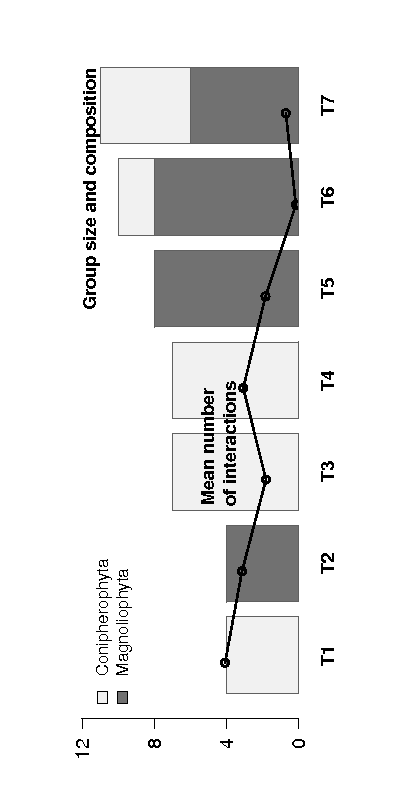
\includegraphics[height=.3\textwidth,width=.35\textwidth,angle=270,origin=c,trim=0 20 0 0]{\fignet/MRV10_AoAS_Q7_group}

  \end{tabular}

}

%====================================================================
\frame{\frametitle{Tree interaction network (2/2)}

  \bigskip
  \begin{tabular}{cc}
    \begin{tabular}{p{.5\textwidth}}
      \paragraph{Additional information:}  ('covariate')  \\ 
      $d_{ij} =$ taxonomic distance between  \\
      species $i$ and $j$ (count) \\
      ~ \\
      \paragraph{Block model:} $K$ groups, 
      $$
      (Y_{ij} \mid Z_i=k, Z_j=\ell) \sim \Pcal(e^{\alpha_{k\ell} + \emphase{\beta d_{ij}}})
      $$
    \end{tabular}
    &
    \pause 
    \begin{tabular}{p{.35\textwidth}}
      $\beta =$ effect of the distance on the number of shared parasites:
      $$ \widehat{\beta} = -.417 $$
      ~ \\
      $\alpha_{k\ell} =$ 'residual' block structure not explained by the distance
    \end{tabular}
  \end{tabular}

  \begin{tabular}{ccc}
    \includegraphics[height=.3\textwidth,width=.3\textwidth]{\fignet/Tree-ICL-SBMall}
    &
    \includegraphics[height=.3\textwidth,width=.3\textwidth]{\fignet/Tree-adjMat-SBMtaxo}
    &
    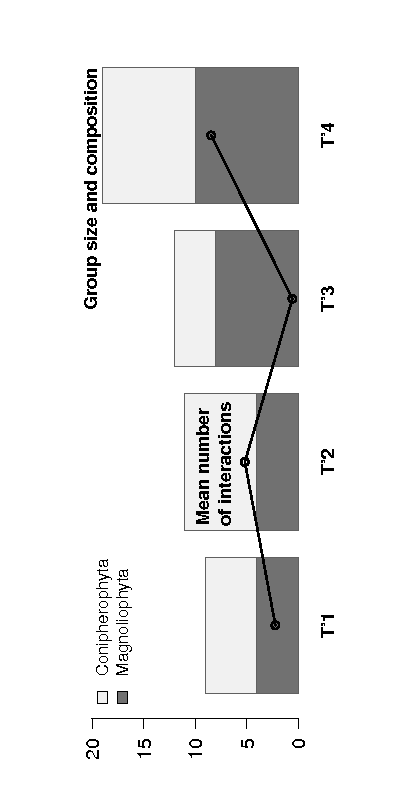
\includegraphics[height=.3\textwidth,width=.35\textwidth,angle=270,origin=c,trim=0 20 0 0]{\fignet/MRV10_AoAS_Q4_group}

  \end{tabular}
}

%====================================================================
\frame{\frametitle{Many block models}

  \begin{description}
   \item[Symmetric] 'stochastic' block model (SBM: \refer{HoL79}) \\ ~
   \item[Valued] or 'weighted' \refer{MRV10} \\ ~ 
   \item[Dynamic] when interaction are collected along time \refer{MaM16} \\ ~
   \item[Overlapping] when individual may belong to several groups ('mixed-membership' : \refer{ABF08,LBA11}) \\ ~
   \item[Multiplex] when different types of interactions are considered \refer{BDL17}
  \end{description}
  
  \bigskip \bigskip 
  \begin{itemize}
   \item Each of them requires specific methodological developments (both theory and code: \url{blockmodels}, \url{dynsbm}, \url{missSBM}, \dots)
  \end{itemize}

}

%====================================================================
%====================================================================
\section[Poisson log-normal model]{Poisson log-normal model as a joint species distribution model}
\frame{\frametitle{Outline} \tableofcontents[currentsection]}
%====================================================================
\frame{\frametitle{Back to Barents' fishes}

  \paragraph{Why model-based?} Model comparison:
  
  \bigskip 
  \begin{tabular}{c|cc}
    \multicolumn{1}{l|}{\emphase{Null model}} & 
    \multicolumn{2}{l}{\emphase{Full model}} \\
    & & \\
    \multicolumn{1}{c|}{{$Y_{ij} \sim \Pcal(\exp(\mu_j + Z_{ij}))$}} & 
    \multicolumn{2}{c}{{$Y_{ij} \sim \Pcal(\exp(x_i^\intercal \beta_j + Z_{ij}))$}} \\
    & & \\
    \multicolumn{1}{l|}{{no covariates}} & 
    \multicolumn{2}{l}{{$x = $ lat., long., depth, temp.}} \\
    & & \\
    inferred correlations $\widehat{\Sigma}_{\text{null}}$ & predicted correlations & inferred  correlations $\widehat{\Sigma}_{\text{full}}$ \\
    \includegraphics[width=.3\textwidth, trim=25 25 25 25]{\figeco/BarentsFish-corrNull} &
    \includegraphics[width=.3\textwidth, trim=25 25 25 25]{\figeco/BarentsFish-corrPred} &
    \includegraphics[width=.3\textwidth, trim=25 25 25 25]{\figeco/BarentsFish-corrAll} 
  \end{tabular}

  }
  
%====================================================================
\frame{\frametitle{Various Poisson log-normal models}

  \paragraph{PLN model \refer{AiH89}.} For each site $i$ and species $j$
  \begin{itemize}
   \item $Z_i \sim \Ncal(0, \Sigma)$: dependencies between species = biotic interactions \\~
   \item $Y_{ij} \sim \Pcal(\exp(o_{ij} + x_i^\intercal \beta_j + Z_{ij}))$: \\ ~\\
    \ra sampling effort ('offset' term $o_{ij}$) \\
    \ra effect of the environmental covariates ($x_i^\intercal \beta_j$: abiotic interactions) \\
    \ra dependency with respect to other species ($Z_{ij}$)
  \end{itemize}
  
  \bigskip
  \paragraph{Confortable framework} to model dependency taking advantage of the Gaussian properties: \\~ 
  \begin{description}
   \item[Principal component analysis (PCA):] assume that $\Sigma$ has rank $q \ll p$ \refer{CMR18} \\~ 
   \item[Network inference:] assume that $\Sigma^{-1}$ is sparse \refer{CMR19}
  \end{description}
  
  \bigskip
  \ra \url{PLNmodels} R package
}
  
%====================================================================
\frame{\frametitle{Dimension reduction in metagenomics}

  \begin{tabular}{ccc}
%    \hspace{-0.05\textwidth}
   \paragraph{Oak powdery mildew.} \refer{JFS16} &
   \paragraph{Without covariates} & 
   \paragraph{With covariates} \\
%    \hspace{-0.05\textwidth}
   \begin{tabular}{p{.3\textwidth}}
      $n = 116$ leaves, \\~ \\
      $p = 114$ OTUs \\
      (bacteria + fungi) \\~ \\
      Different sampling efforts for bacteria and fungi \\~ \\
      Several covariates, \\~ \\
      inc. tree status: \textcolor{blue}{susceptible}, \textcolor{red}{intermediate}, \textcolor{green}{resistant}
    \end{tabular}
    &
    \hspace{-0.05\textwidth}
    \begin{tabular}{c}
      \includegraphics[width=.3\textwidth]{\figeco/CMR18-Fig4a1} \\ ~\\
      \includegraphics[width=.3\textwidth]{\figeco/CMR18-Fig5a1}
    \end{tabular}
    &
    \hspace{-0.05\textwidth}
    \begin{tabular}{c}
      \includegraphics[width=.3\textwidth]{\figeco/CMR18-Fig4a2} \\ ~\\
      \includegraphics[width=.3\textwidth]{\figeco/CMR18-Fig5a2}
    \end{tabular}
  \end{tabular}

  }
  

%====================================================================
%====================================================================
\backupbegin 
\section*{Backup}
%====================================================================
\frame[allowframebreaks]{ \frametitle{References}
  {%\footnotesize
   \tiny
   \bibliography{/home/robin/Biblio/BibGene}
%    \bibliographystyle{/home/robin/LATEX/Biblio/astats}
   \bibliographystyle{alpha}
  }
}

%====================================================================
\frame{\frametitle{Tree interaction network}

  \paragraph{Residual structure.} Rather than choosing an optimal number of group $K$, average over all block structures \refer{LaR16,DoR19}

  \bigskip
  \begin{centering}
    \begin{tabular}{ccc}
      Model weights & Averaged residual structure & Species identification \\
      \includegraphics[height=.3\textwidth,width=.3\textwidth]{\fignet/Tree-all-V10-M5000-logpY} &
      \includegraphics[height=.3\textwidth,width=.3\textwidth,trim=60 60 60 60]{\fignet/Tree-all-V10-M5000-graphon} &
      \includegraphics[height=.3\textwidth,width=.3\textwidth]{\fignet/Tree-all-V10-M5000-Ui-neighbours}
    \end{tabular}
  \end{centering}

}

%====================================================================
\frame{\frametitle{Barents fish} 

  \begin{center}
  \begin{tabular}{lccc}
    & no covariate & \textcolor{blue}{temp. \& depth} & \textcolor{red}{all covariates} \\
    \hline
    \rotatebox{90}{$\qquad\quad\lambda=.20$} &
    \includegraphics[width=.22\textwidth]{\figCMR/network_BarentsFish_Gnull_full60edges} &
    \includegraphics[width=.22\textwidth]{\figCMR/network_BarentsFish_Gsel_full60edges} &
    \includegraphics[width=.22\textwidth]{\figCMR/network_BarentsFish_Gfull_full60edges} 
    \vspace{-0.05\textheight} \\ \hline
    %
    \rotatebox{90}{$\qquad\quad\lambda=.28$} &
    \includegraphics[width=.22\textwidth]{\figCMR/network_BarentsFish_Gnull_sel60edges} & \includegraphics[width=.22\textwidth]{\figCMR/network_BarentsFish_Gsel_sel60edges} &
    \includegraphics[width=.22\textwidth]{\figCMR/network_BarentsFish_Gfull_sel60edges} 
    \vspace{-0.05\textheight} \\ \hline
    %
    \rotatebox{90}{$\qquad\quad\lambda=.84$} &
    \includegraphics[width=.22\textwidth]{\figCMR/network_BarentsFish_Gnull_null60edges} &
    \includegraphics[width=.22\textwidth]{\figCMR/network_BarentsFish_Gsel_null60edges} &
    \includegraphics[width=.22\textwidth]{\figCMR/network_BarentsFish_density} 
%     \includegraphics[width=.22\textwidth]{\figCMR/network_BarentsFish_Gfull_null60edges}  
  \end{tabular}
  \end{center}

}

%====================================================================
\backupend 

%====================================================================
%====================================================================
\end{document}
%====================================================================
%====================================================================

  \begin{tabular}{cc}
    \begin{tabular}{p{.5\textwidth}}
    \end{tabular}
    &
    \begin{tabular}{p{.45\textwidth}}
    \end{tabular}
  \end{tabular}

